\chapter{Estado da Arte}

\section{Introdução}

O presente capítulo tem como finalidade apresentar o estado da arte relativo à temática em análise, reunindo e examinando criticamente as principais contribuições científicas e jogos desenvolvidas até ao momento. A compreensão do panorama atual do conhecimento revela-se fundamental para enquadrar o projeto.

Neste capítulo serão, assim, analisados um conjunto de jogos e artigos, procurando estabelecer um enquadramento crítico que permita compreender a evolução do conhecimento na área e sustentar o desenvolvimento apresentado nos capítulos subsequentes.

\section{Vídeo Jogos}

\subsection{Data Center Demo}

\begin{figure}[H]
\centering
\begin{tabular}{ll}

\begin{minipage}{0.55\textwidth}
\textcite{DataCenterDemo} está a desenvolver o jogo
    Data Center (ver Figura \ref{DataCenter_Capa}), que atualmente está em versão Demo na Steam
    e com previsão de lançamento para
    o dia 31 de março de 2026, é um jogo do estilo simulador técnico que foca na representação tridimensional e na gestão de infraestruturas de TI. Ao contrário de jogos puramente recreativos, a sua prioridade é a fidelidade técnica e a visualização de métricas em tempo real.
    Alguns dos pontos mais explorados por ele são:
\end{minipage}
&
\begin{minipage}{0.35\textwidth}
\centering

\includegraphics[width=\textwidth]{images/DataCenterCapa.jpg}
\caption[Data Center Demo - Capa do jogo. Retirado de \url{https://store.steampowered.com/app/4376050/Data_Center_Demo}]{Data Center Demo - Capa do jogo.}
\label{DataCenter_Capa}
\end{minipage}
\end{tabular}
\end{figure}


\begin{itemize}
  \item Gestão de Infraestrutura Física:
  Apresenta para o jogador a disposição das \textit{racks}, unidades de distribuição de energia (PDUs) e sistemas de arrefecimento (CRACs). Demonstrando como o layout físico impacta diretamente a eficiência operacional (ver Figura \ref{DataCenter_Gameplay1}).
O jogador terá de fazer a instalação de uma infraestrutura passando pela várias etapas, como montagem, conexão de cabos e configuração de equipamentos.
  \begin{figure}[h]
    \centering
    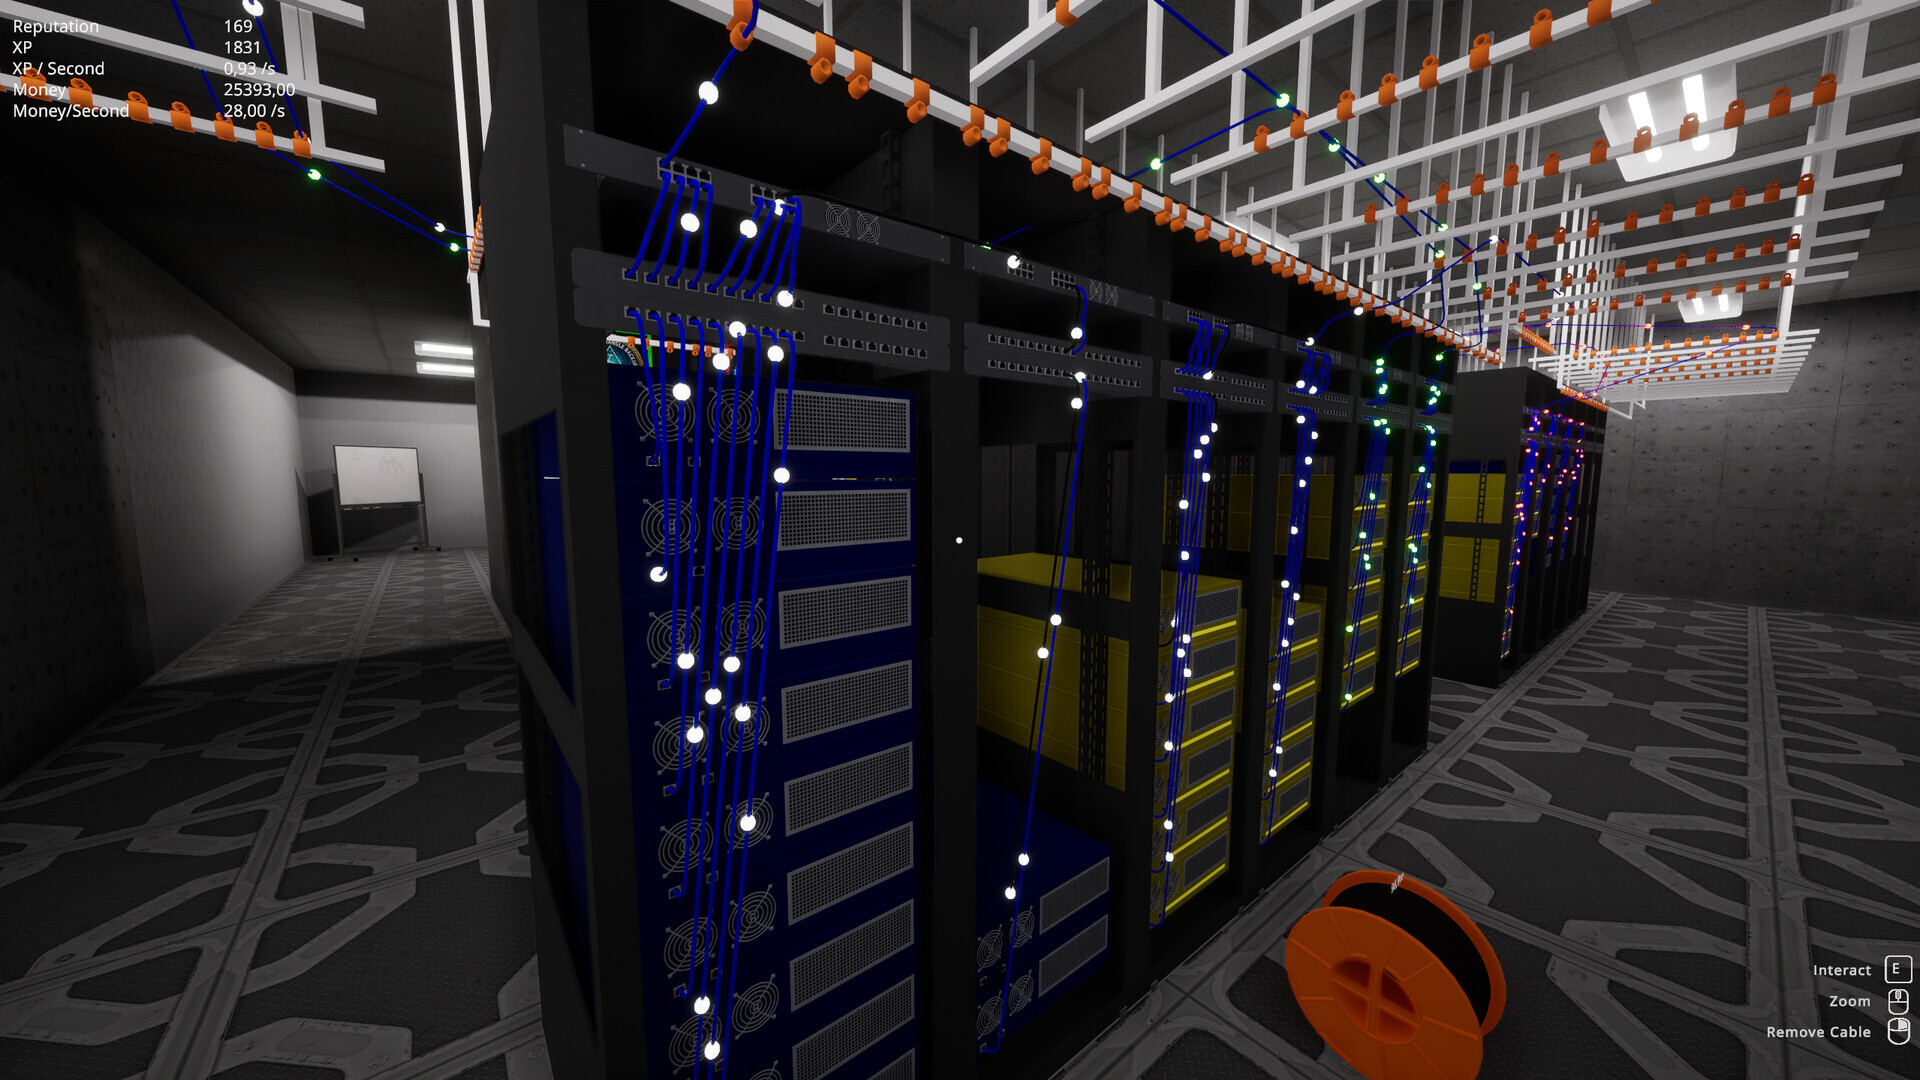
\includegraphics[width=0.8\textwidth]{images/DataCenter1.jpg}
    \caption[Data Center Demo - Configuração de \textit{racks}, ligação de cabos. Retirado de \url{https://store.steampowered.com/app/4376050/Data_Center_Demo}]{Data Center Demo - Configuração de racks, ligação de cabos.}
    \label{DataCenter_Gameplay1}
  \end{figure}
  \item Visualização Térmica:
  Uma das funcionalidades mais marcantes é a simulação de fluxo de ar e calor. O "jogo" mostra visualmente o impacto de corredores quentes e frios, permitindo que o jogador identifique \textit{hotspots} que poderiam levar à falha do \textit{hardware}.
  \item Simulação de Carga e Falhas:
  Permite ao jogador simular picos de tráfego ou falhas em componentes específicos (como a queda de um gerador ou UPS) para observar como o sistema de redundância reage.
  \item Métricas de Sustentabilidade:
  O \textit{software} calcula e apresenta indicadores de desempenho como o PUE (Power Usage Effectiveness).
\end{itemize}

\vspace{0.5cm}

O projeto desenvolvido apresenta diversas semelhanças com o Data Center Demo, nomeadamente ao nível do contexto de jogo, da tipologia de objetos representados e do cenário. Contudo, essas características são retratadas de forma mais simplificada e incluem alguns elementos de fantasia. A principal intenção é privilegiar a componente lúdica e a experiência de entretenimento, sem, no entanto, excluir por completo os elementos técnicos subjacentes à simulação.

\subsection{PC Building Simulator}

\begin{figure}[H]
\centering
\begin{tabular}{ll}

\begin{minipage}{0.55\textwidth}
\textcite{PCBuildingSimulator} desenvolveu o PC Building Simulator (ver Figura \ref{PCBuild_Capa}) com a proposta de ser um jogo de montagem de computadores, que permite ao jogador passar pelas várias etapas de montagem de um computador pessoal. O jogo destaca-se pela representação fiel de componentes e pela introdução de conceitos técnicos como compatibilidade de \textit{sockets}.
\end{minipage}
&
\begin{minipage}{0.35\textwidth}
\centering
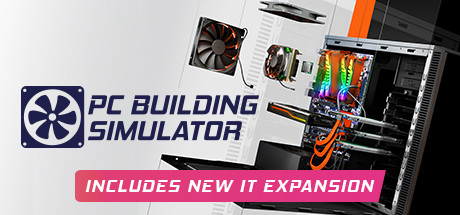
\includegraphics[width=\textwidth]{images/PCBuildSimulator-Header.jpg}
\caption[PC Building Simulator - Capa do jogo. Retirado de \url{https://store.steampowered.com/app/621060/PC_Building_Simulator}]{PC Building Simulator - Capa do jogo. }
\label{PCBuild_Capa}
\end{minipage}
\end{tabular}
\end{figure}

\begin{itemize}
    \item Instalação de \textit{hardware}, desde da colocação de \textit{hardware} até conexão de cabos;
    \item Instalação de sistemas operativos;
    \item Instalação de \textit{softwares} adicionais e realização de teste.
\end{itemize}

O jogo destaca-se pela representação fiel de componentes (CPU,GPU,RAM,etc...) e pela
introdução de conceitos técnicos como compatibilidade de \textit{sockets} (ver Figura \ref{PCBuild_Gameplay1}).

\begin{figure}[H]
  \centering
  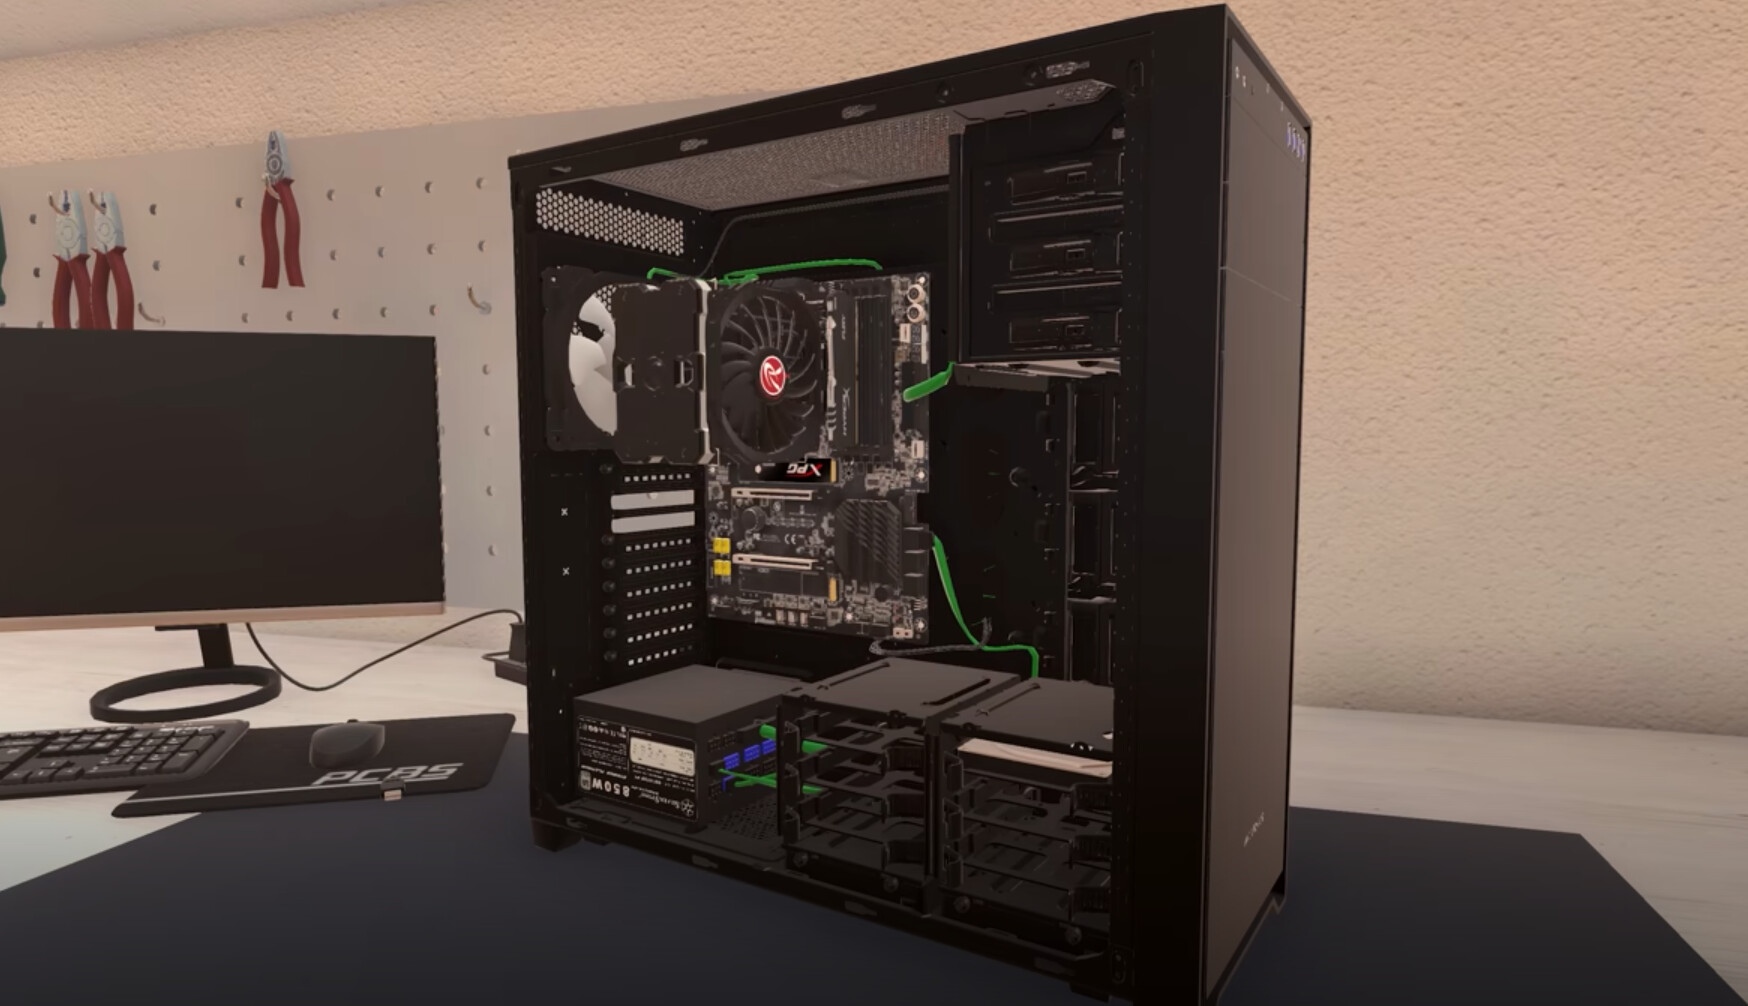
\includegraphics[width=0.8\textwidth]{images/PCBuildSimulator_BuildPC.jpg}
  \caption[PC Building Simulator - Montagem de um computador. Retirado de \url{https://store.steampowered.com/app/621060/PC_Building_Simulator}]{PC Building Simulator - Montagem de um computador.}
  \label{PCBuild_Gameplay1}
\end{figure}

A representação realista do hardware, bem como a simulação da instalação de sistemas operativos, foram também retratadas no projecto desenvolvido, ainda que de forma mais simplificada, lúdica e adaptada ao respectivo contexto.
Importa salientar que, à data da redação deste texto, já se encontra disponível o PC Building Simulator 2. No entanto, para efeitos deste trabalho, os aspetos apresentados são comuns a ambas as versões.

\subsection{Startup Company}

\begin{figure}[H]
\centering
\begin{tabular}{ll}
\begin{minipage}{0.55\textwidth}
\textcite{StartupCompany} desenvolveu o jogo Startup Company (ver Figura \ref{StartUP_Capa}), que apresenta uma proposta centrada na simulação de gestão empresarial na área da tecnologia. Neste jogo, o jogador assume a responsabilidade de criar e desenvolver uma empresa tecnológica a partir do zero , gerindo recursos materiais e humanos.
\end{minipage}
&
\begin{minipage}{0.35\textwidth}
\centering

\includegraphics[width=\textwidth]{images/StartUPCompany_Header.jpg}
\caption[Startup Company - Capa do jogo. Retirado de \url{https://store.steampowered.com/app/606800/Startup_Company/?l=portuguese}]{Startup Company - Capa do jogo. }
\label{StartUP_Capa}
\end{minipage}
\end{tabular}
\end{figure}

Compete-lhe gerir de forma estratégica os recursos materiais (ver Figura \ref{StarUP_Server}), nomeadamente os espaços e o local de trabalho, bem como os recursos humanos, incluindo programadores, líderes de projeto, designers, profissionais de marketing e responsáveis pela gestão de servidores (ver Figura \ref{StartUP_RH}).

\begin{figure}[H]
  \centering
  % --- Primeira Figura (Métricas) ---
  \begin{minipage}[b]{0.48\textwidth}
    \centering
    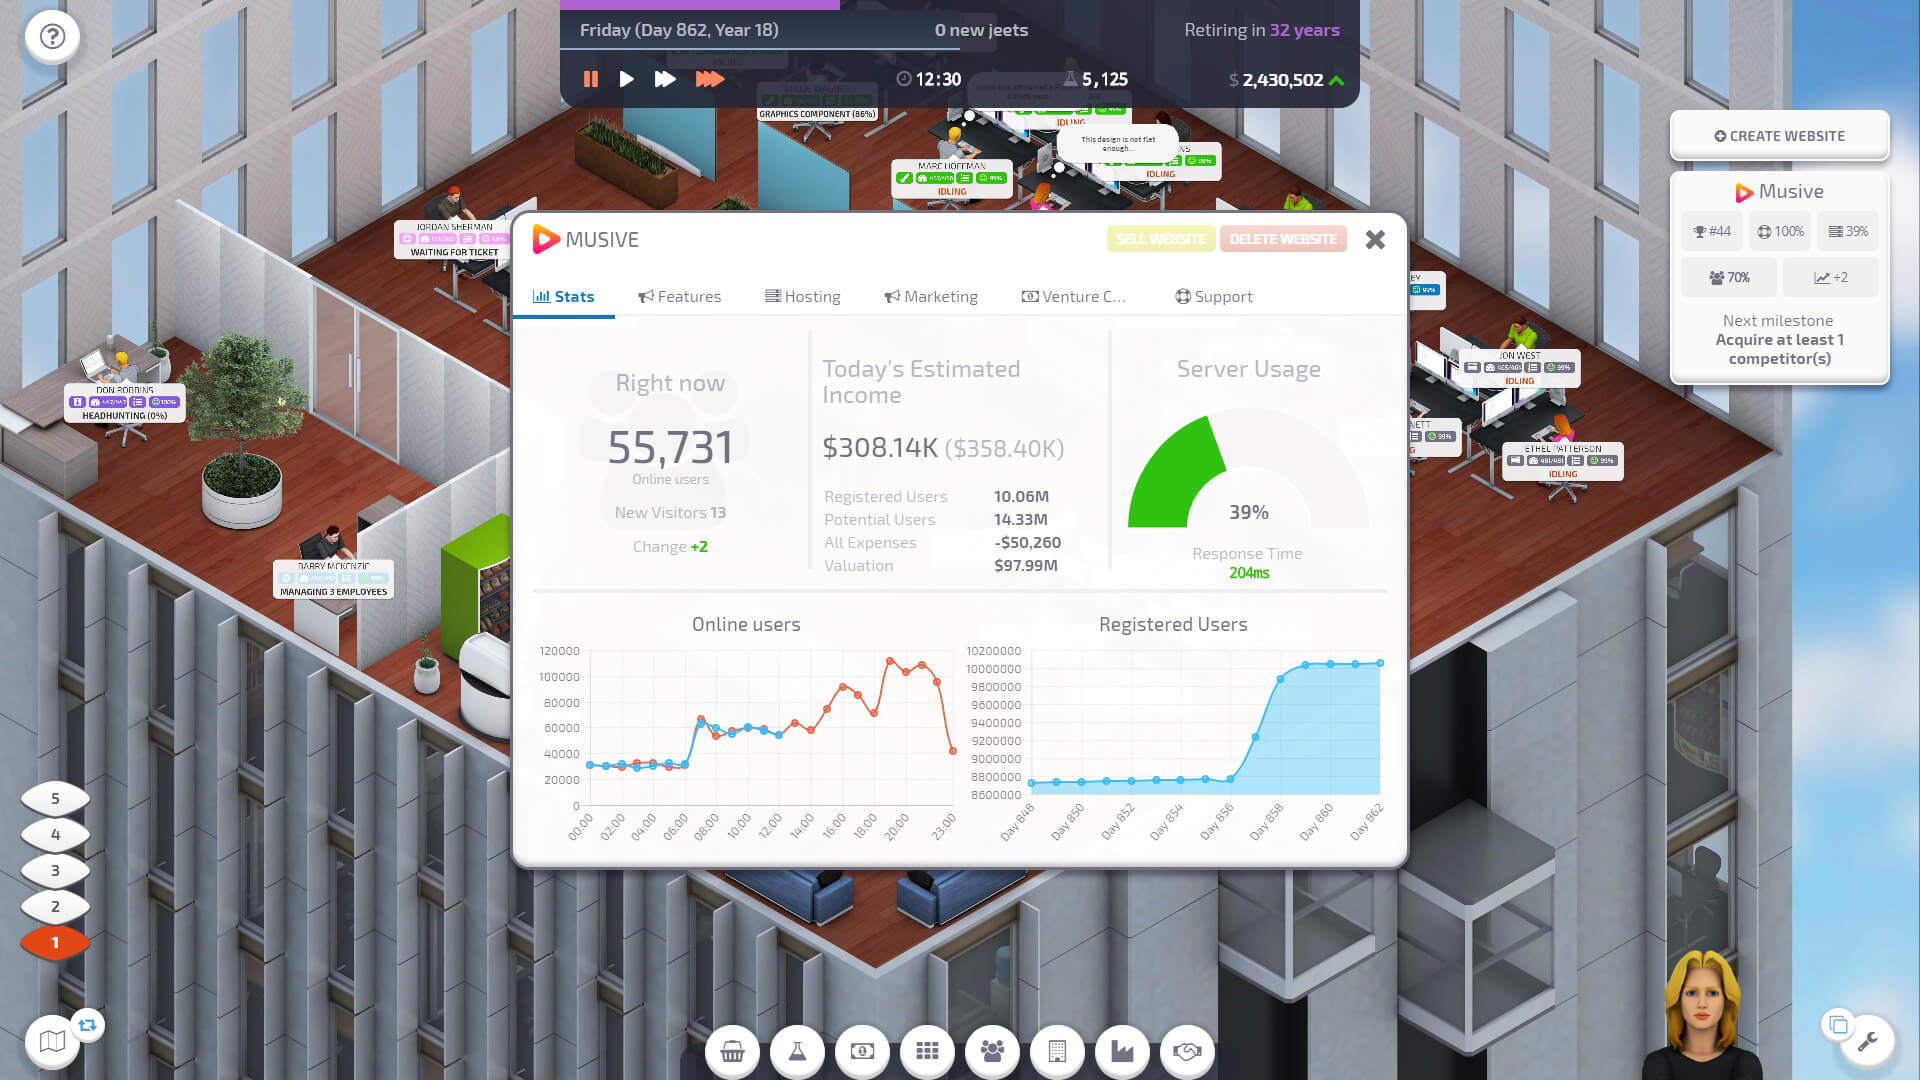
\includegraphics[width=\textwidth]{images/Startup-Metrics.jpg}
    \caption[Startup Company - Métricas que o jogo disponibiliza para o jogador. Retirado de \url{https://store.steampowered.com/app/606800/Startup_Company/?l=portuguese}]{Startup Company - Métricas que o jogo disponibiliza para o jogador.}
    \label{StartUP_Dinheiro}
  \end{minipage}
  \hfill % Espaçamento entre as minipages
  % --- Segunda Figura (Servidores) ---
  \begin{minipage}[b]{0.48\textwidth}
    \centering
    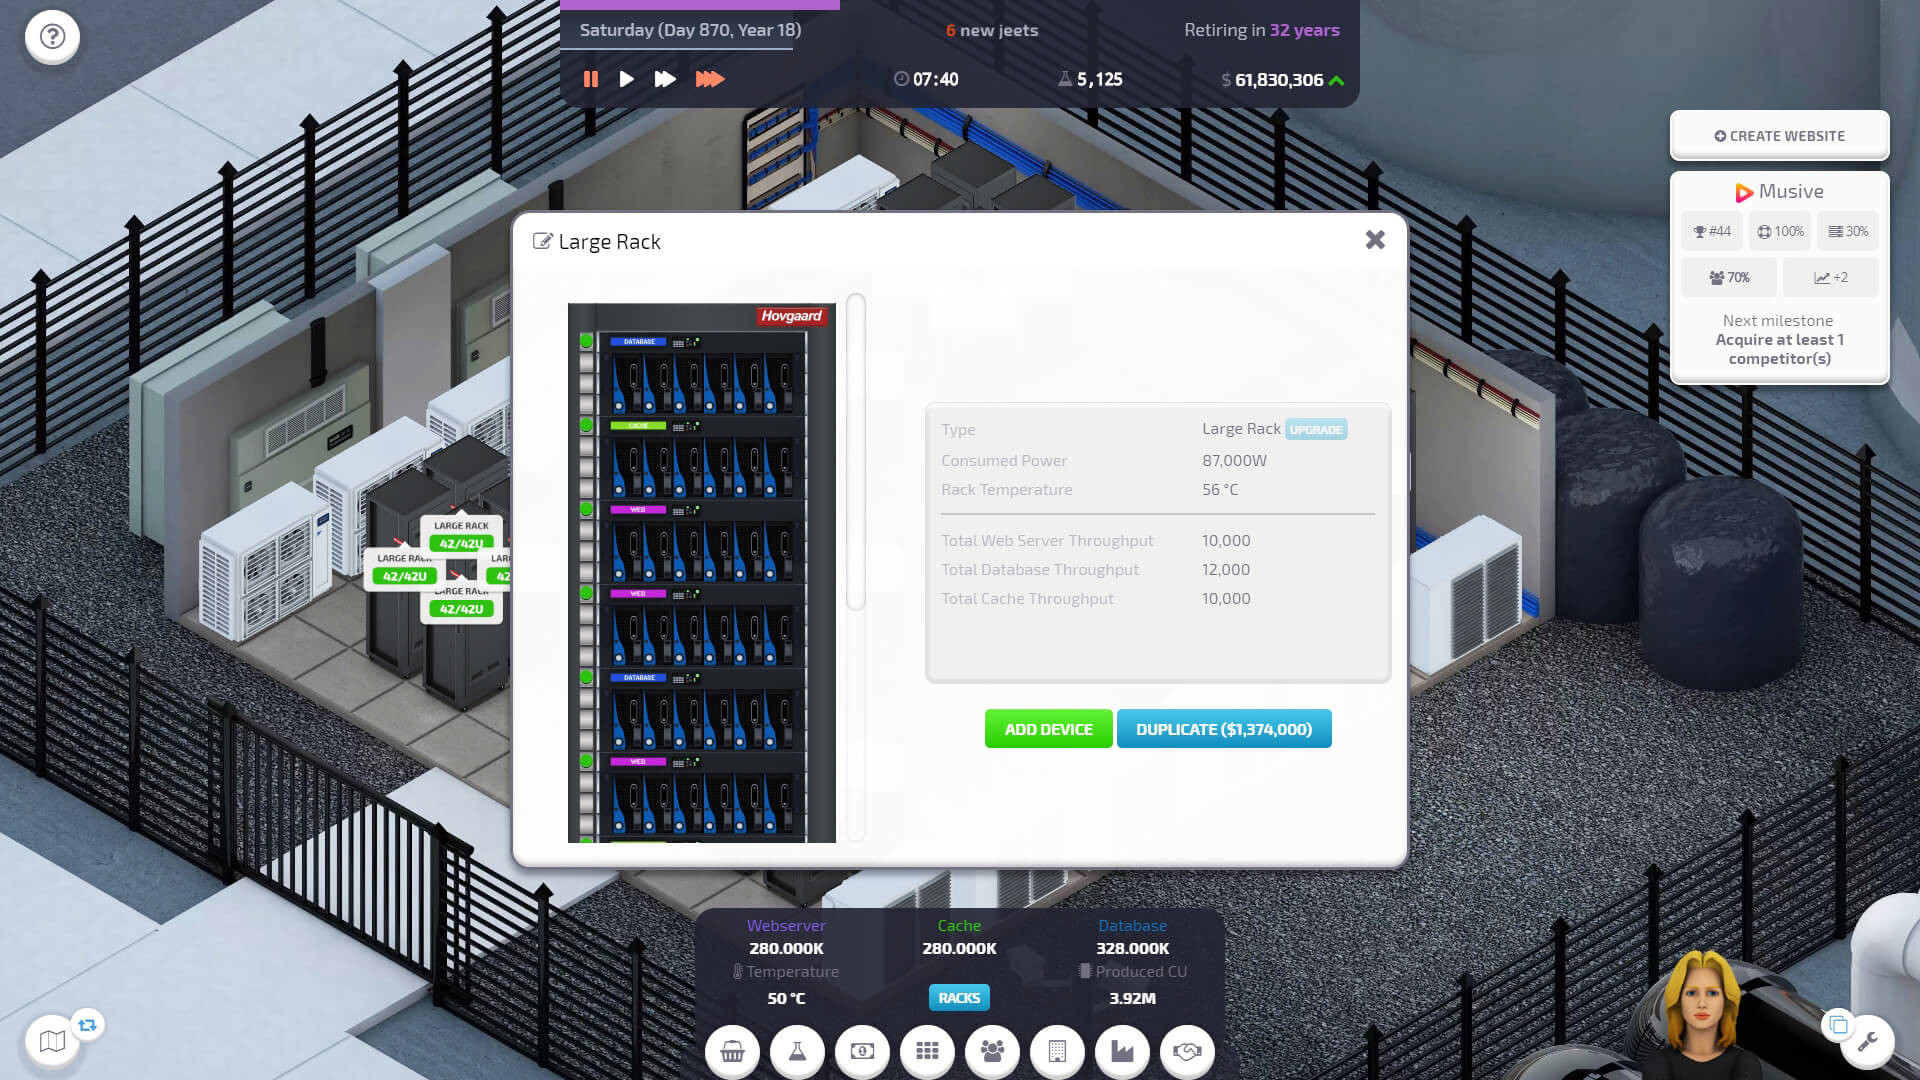
\includegraphics[width=\textwidth]{images/Startup-Server.jpg}
    \caption[Startup Company - Configurações de servidores. Retirado de \url{https://store.steampowered.com/app/606800/Startup_Company/?l=portuguese}]{Startup Company - Configurações de servidores.}
    \label{StarUP_Server}
  \end{minipage}
\end{figure}

\begin{figure}[H]
  \centering
  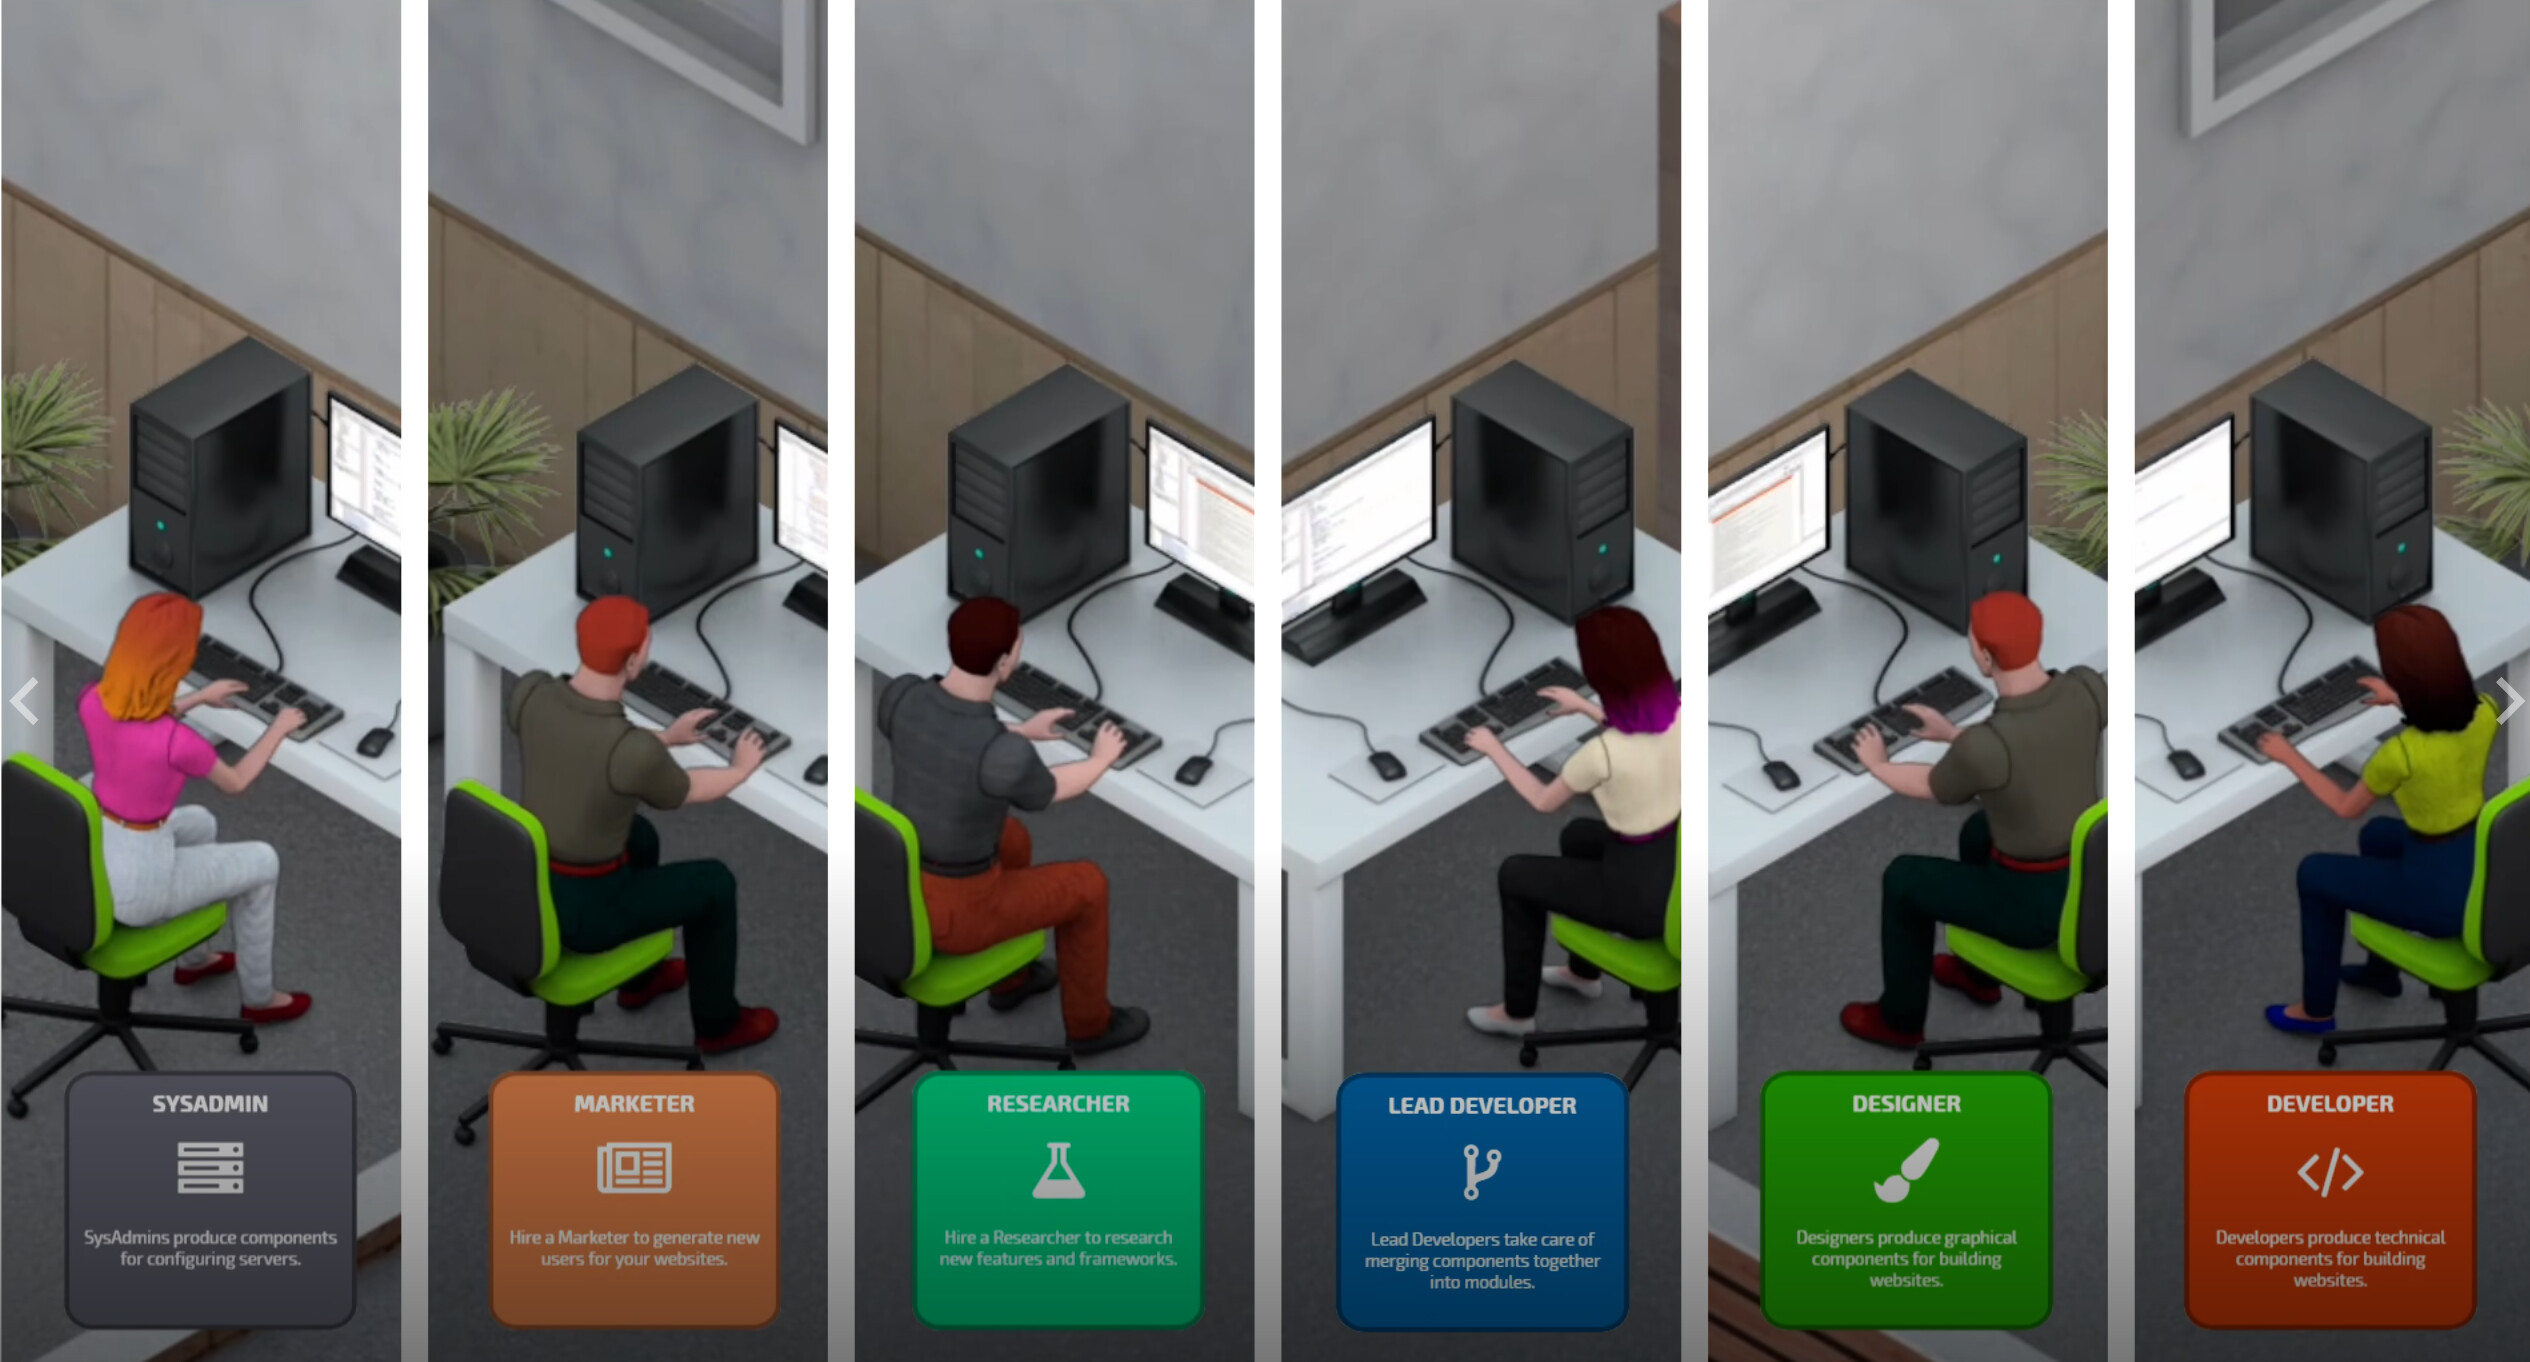
\includegraphics[width=0.6\textwidth]{images/Startu - humanos.jpg}
  \caption[Startup Company - Exemplo de recursos humanos disponiveis. Retirado de \url{https://store.steampowered.com/app/606800/Startup_Company/?l=portuguese}]{Startup Company - Exemplo de recursos humanos disponiveis. Retirado de \url{https://store.steampowered.com/app/606800/Startup_Company/?l=portuguese}}
  \label{StartUP_RH}
\end{figure}

Além dessa parte, gestão de cliente, custo, consumos da infraestrutura assim como rendimentos, são fatores relavantes
neste jogo (ver Figura \ref{StartUP_Dinheiro}). Serviram de inspiração para a criação de funcionalidades no projeto, tais como
pedido de serviços feito por clientes para o jogador, e métricas de consumo e desempenho.


\subsection{Grey Hack}

\begin{figure}[H]
\centering
\begin{tabular}{ll}
\begin{minipage}{0.55\textwidth}
\textcite{GreyHarck} está a desenvolver o jogo Grey Hack (ver Figura \ref{GreyHack_Capa}), o qual está em acesso antecipado na plataforma Steam. Estes títulos focam-se na simulação de ambientes de rede e \textit{hacking} por interfaces que mimetizam sistemas operativos reais , utilizando terminais de linha de comando (CLI).
\end{minipage}
&
\begin{minipage}{0.35\textwidth}
\centering

\includegraphics[width=\textwidth]{images/GreyHack-Header.jpg}
\caption[Grey Hack - Capa do jogo. Retirado de \url{https://store.steampowered.com/app/605230/Grey_Hack}]{Grey Hack - Capa do jogo. }
\label{GreyHack_Capa}
\end{minipage}
\end{tabular}
\end{figure}

Grey Hack utiliza terminais de linha de comando (CLI) e visualizações de 
topologia de rede para criar uma experiência imersiva, onde o jogador interage 
com o sistema de forma lógica e textual (ver Figura \ref{GreyHack_UI}).

\begin{figure}[H]
  \centering
  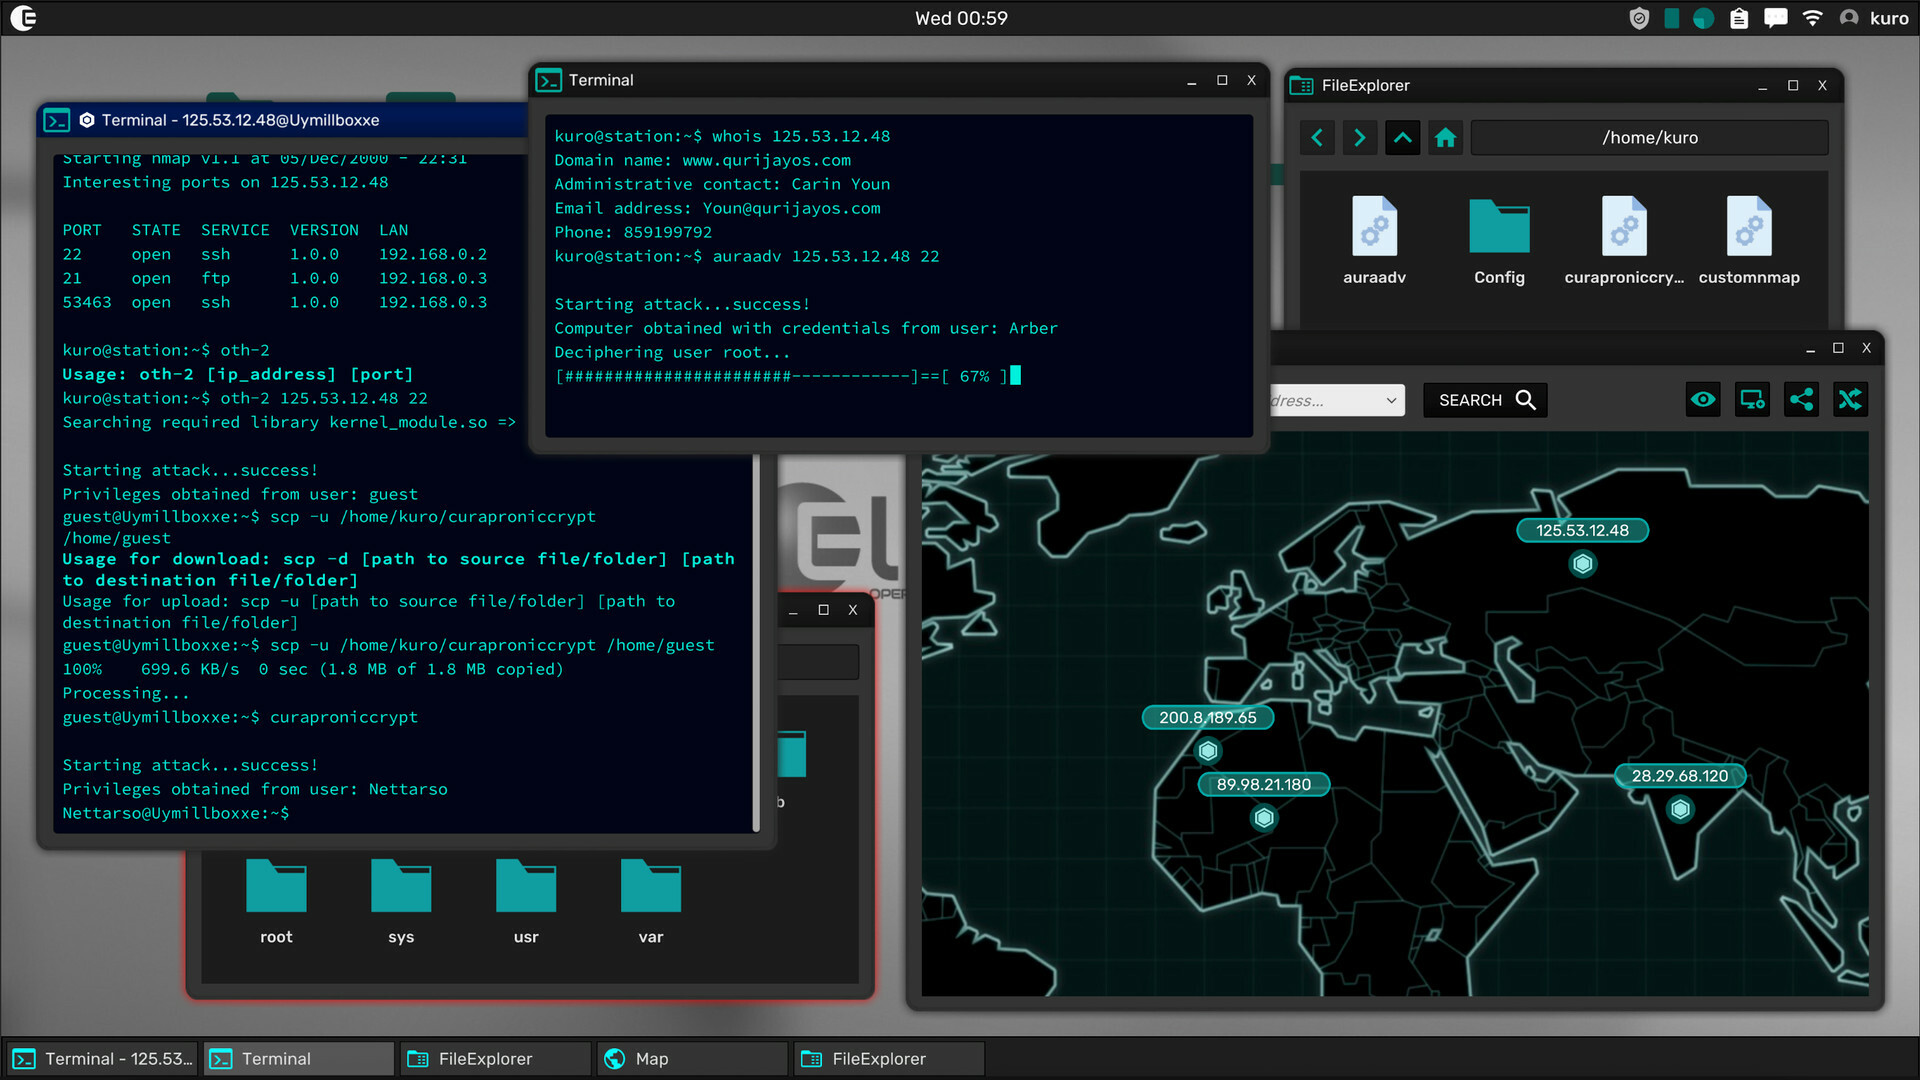
\includegraphics[width=\textwidth]{images/Grey Hack - Terminal.jpg}
  \caption[Grey Hack - UI de terminal. Retirado de \url{https://store.steampowered.com/app/605230/Grey_Hack}]{Grey Hack - UI de terminal. Retirado de \url{https://store.steampowered.com/app/605230/Grey_Hack}}
  \label{GreyHack_UI}
\end{figure}

Transpondo para o projeto, estas referências servem de base para a camada de interação (UI/UX). 
O projeto adota a utilização de terminais virtuais para a conclusão de \textit{mini games}.

\subsection{Software Inc.}

\begin{figure}[H]
\centering
\begin{tabular}{ll}
\begin{minipage}{0.55\textwidth}
\textcite{SoftwareInc} desenvolveu o jogo Software Inc. (ver Figura \ref{SoftwareInc_Capa}), o qual apresenta um sistema de construção complexo que inclui a gestão de eletricidade, temperatura e disposição de salas. O jogo exige que o jogador planeie a colocação de sistemas de arrefecimento e geradores para garantir a integridade do hardware.
\end{minipage}
&
\begin{minipage}{0.35\textwidth}
\centering
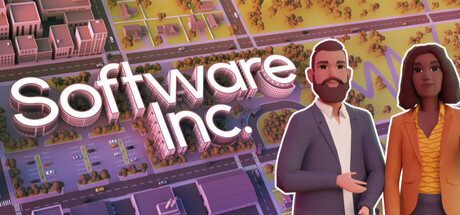
\includegraphics[width=\textwidth]{images/SoftwareInc-Header.jpg}
\caption[Software Inc - Capa do jogo. Retirado de \url{https://store.steampowered.com/app/362620/Software_Inc}]{Software Inc - Capa do jogo. }
\label{SoftwareInc_Capa}
\end{minipage}
\end{tabular}
\end{figure}

A influência de Software Inc. no projeto reside no planeamento de sistemas. Tais como a necessidade 
de gerir a gestão da rede elétrica (capacidade das UPS e geradores) são mecânicas de logística urbana adaptadas 
para o ambiente de jogo.

\section{Artigos científicos}
Para além dos videojogos anteriormente referenciados, existe um conjunto de artigos que 
se enquadram na área científica do projeto e que foram fundamentais para sustentar o seu 
desenvolvimento, estabelecendo uma ponte importante entre o universo dos jogos e a aplicação 
real. Um exemplo desta correlação é o trabalho de \textcite{Gametheory-DataCenters}, que demonstra 
como conceitos teóricos complexos, como a Teoria dos Jogos, são aplicados na prática para 
identificar centros de dados vulneráveis em redes de computação em nuvem através da análise 
de custos e tempos de resposta. A inclusão desta referência no estado da arte serve para 
validar como as dinâmicas de gestão e os desafios de infraestrutura abordados no projeto 
refletem preocupações reais e atuais da computação científica, reforçando a relevância 
do contexto em que o utilizador é inserido.

\todo{Revisar}

A metodologia de design é apoiada por \textcite{SeriousGames-Frutuoso}, que descreve diretrizes para a 
criação de jogos com objetivos educacionais. Embora o projeto desenvolvido não se define 
como um jogo sério, a metodologia
 apresentada foi relevante na fase de conceptualização para estruturar a integração de 
 conteúdos técnicos de forma equilibrada. Esta abordagem é complementada pelos conceitos 
 de macrodesign de \textcite{shay2022scaffolding}, que identificam fatores cruciais como a 
 fantasia, o mistério e o desafio para garantir que o rigor do tema não prejudica a imersão 
 lúdica. Para o desenvolvimento deste trabalho, a aplicação destes fatores justifica a 
 inclusão de elementos de fantasia e métricas simplificadas em cima de conhecimentos 
 reais, garantindo que o jogador se mantenha motivado por mecânicas envolventes 
 e permitindo a criação de um conceito de jogo que soma conhecimentos ao jogador mantendo 
 a diversão como fator principal.

Por fim estudo como, \textit{Video Games and Indirect Learning: A Study of 12 Games That Can Teach} realizado
por Monica \textcite{miller2021video} defende que video jogos meramente comerciais, ou
seja jogos que não são focados em transmitir conhecimentos como é o caso de jogos sérios,
 conseguem transmitir conhecemintos ao jogo.

\todo{Aqui}